\documentclass[twoside]{book}

% Packages required by doxygen
\usepackage{calc}
\usepackage{doxygen}
\usepackage{graphicx}
\usepackage[utf8]{inputenc}
\usepackage{makeidx}
\usepackage{multicol}
\usepackage{multirow}
\usepackage{textcomp}
\usepackage[table]{xcolor}

% Font selection
\usepackage[T1]{fontenc}
\usepackage{mathptmx}
\usepackage[scaled=.90]{helvet}
\usepackage{courier}
\usepackage{amssymb}
\usepackage{sectsty}
\renewcommand{\familydefault}{\sfdefault}
\allsectionsfont{%
  \fontseries{bc}\selectfont%
  \color{darkgray}%
}
\renewcommand{\DoxyLabelFont}{%
  \fontseries{bc}\selectfont%
  \color{darkgray}%
}

% Page & text layout
\usepackage{geometry}
\geometry{%
  a4paper,%
  top=2.5cm,%
  bottom=2.5cm,%
  left=2.5cm,%
  right=2.5cm%
}
\tolerance=750
\hfuzz=15pt
\hbadness=750
\setlength{\emergencystretch}{15pt}
\setlength{\parindent}{0cm}
\setlength{\parskip}{0.2cm}
\makeatletter
\renewcommand{\paragraph}{%
  \@startsection{paragraph}{4}{0ex}{-1.0ex}{1.0ex}{%
    \normalfont\normalsize\bfseries\SS@parafont%
  }%
}
\renewcommand{\subparagraph}{%
  \@startsection{subparagraph}{5}{0ex}{-1.0ex}{1.0ex}{%
    \normalfont\normalsize\bfseries\SS@subparafont%
  }%
}
\makeatother

% Headers & footers
\usepackage{fancyhdr}
\pagestyle{fancyplain}
\fancyhead[LE]{\fancyplain{}{\bfseries\thepage}}
\fancyhead[CE]{\fancyplain{}{}}
\fancyhead[RE]{\fancyplain{}{\bfseries\leftmark}}
\fancyhead[LO]{\fancyplain{}{\bfseries\rightmark}}
\fancyhead[CO]{\fancyplain{}{}}
\fancyhead[RO]{\fancyplain{}{\bfseries\thepage}}
\fancyfoot[LE]{\fancyplain{}{}}
\fancyfoot[CE]{\fancyplain{}{}}
\fancyfoot[RE]{\fancyplain{}{\bfseries\scriptsize Generated on Thu May 29 2014 12\-:58\-:59 for Lib Bomberman by Doxygen }}
\fancyfoot[LO]{\fancyplain{}{\bfseries\scriptsize Generated on Thu May 29 2014 12\-:58\-:59 for Lib Bomberman by Doxygen }}
\fancyfoot[CO]{\fancyplain{}{}}
\fancyfoot[RO]{\fancyplain{}{}}
\renewcommand{\footrulewidth}{0.4pt}
\renewcommand{\chaptermark}[1]{%
  \markboth{#1}{}%
}
\renewcommand{\sectionmark}[1]{%
  \markright{\thesection\ #1}%
}

% Indices & bibliography
\usepackage{natbib}
\usepackage[titles]{tocloft}
\setcounter{tocdepth}{3}
\setcounter{secnumdepth}{5}
\makeindex

% Hyperlinks (required, but should be loaded last)
\usepackage{ifpdf}
\ifpdf
  \usepackage[pdftex,pagebackref=true]{hyperref}
\else
  \usepackage[ps2pdf,pagebackref=true]{hyperref}
\fi
\hypersetup{%
  colorlinks=true,%
  linkcolor=blue,%
  citecolor=blue,%
  unicode%
}

% Custom commands
\newcommand{\clearemptydoublepage}{%
  \newpage{\pagestyle{empty}\cleardoublepage}%
}


%===== C O N T E N T S =====

\begin{document}

% Titlepage & ToC
\hypersetup{pageanchor=false}
\pagenumbering{roman}
\begin{titlepage}
\vspace*{7cm}
\begin{center}%
{\Large Lib Bomberman \\[1ex]\large 1.\-0 }\\
\vspace*{1cm}
{\large Generated by Doxygen 1.8.6}\\
\vspace*{0.5cm}
{\small Thu May 29 2014 12:58:59}\\
\end{center}
\end{titlepage}
\clearemptydoublepage
\tableofcontents
\clearemptydoublepage
\pagenumbering{arabic}
\hypersetup{pageanchor=true}

%--- Begin generated contents ---
\chapter{Hierarchical Index}
\section{Class Hierarchy}
This inheritance list is sorted roughly, but not completely, alphabetically\+:\begin{DoxyCompactList}
\item \contentsline{section}{A\+Character}{\pageref{class_a_character}}{}
\begin{DoxyCompactList}
\item \contentsline{section}{I\+A}{\pageref{class_i_a}}{}
\item \contentsline{section}{Player}{\pageref{class_player}}{}
\end{DoxyCompactList}
\item \contentsline{section}{A\+Object}{\pageref{class_a_object}}{}
\begin{DoxyCompactList}
\item \contentsline{section}{Cube}{\pageref{class_cube}}{}
\end{DoxyCompactList}
\item \contentsline{section}{tinyxml2\+:\+:Mem\+Pool\+T$<$ S\+I\+Z\+E $>$\+:\+:Block}{\pageref{structtinyxml2_1_1_mem_pool_t_1_1_block}}{}
\item \contentsline{section}{Bomb}{\pageref{class_bomb}}{}
\item \contentsline{section}{Bomberman}{\pageref{class_bomberman}}{}
\item \contentsline{section}{Box\+Bonus}{\pageref{class_box_bonus}}{}
\item \contentsline{section}{Button}{\pageref{class_button}}{}
\item \contentsline{section}{Camera}{\pageref{class_camera}}{}
\item \contentsline{section}{tinyxml2\+:\+:Mem\+Pool\+T$<$ S\+I\+Z\+E $>$\+:\+:Chunk}{\pageref{uniontinyxml2_1_1_mem_pool_t_1_1_chunk}}{}
\item \contentsline{section}{Xml\+Write\+:\+:Controller}{\pageref{class_xml_write_1_1_controller}}{}
\item \contentsline{section}{tinyxml2\+:\+:Dyn\+Array$<$ T, I\+N\+I\+T\+I\+A\+L\+\_\+\+S\+I\+Z\+E $>$}{\pageref{classtinyxml2_1_1_dyn_array}}{}
\item \contentsline{section}{tinyxml2\+:\+:Dyn\+Array$<$ char, 20 $>$}{\pageref{classtinyxml2_1_1_dyn_array}}{}
\item \contentsline{section}{tinyxml2\+:\+:Dyn\+Array$<$ const char $\ast$, 10 $>$}{\pageref{classtinyxml2_1_1_dyn_array}}{}
\item \contentsline{section}{tinyxml2\+:\+:Dyn\+Array$<$ tinyxml2\+:\+:Mem\+Pool\+T\+:\+:Block $\ast$, 10 $>$}{\pageref{classtinyxml2_1_1_dyn_array}}{}
\item exception\begin{DoxyCompactList}
\item \contentsline{section}{Error\+Bomberman}{\pageref{class_error_bomberman}}{}
\end{DoxyCompactList}
\item Game\begin{DoxyCompactList}
\item \contentsline{section}{Game\+Engine}{\pageref{class_game_engine}}{}
\end{DoxyCompactList}
\item \contentsline{section}{Generate\+Maze}{\pageref{class_generate_maze}}{}
\item \contentsline{section}{Generate\+Text}{\pageref{class_generate_text}}{}
\item \contentsline{section}{I\+Game\+State}{\pageref{class_i_game_state}}{}
\begin{DoxyCompactList}
\item \contentsline{section}{Game\+State}{\pageref{class_game_state}}{}
\item \contentsline{section}{Intro\+State}{\pageref{class_intro_state}}{}
\item \contentsline{section}{Load\+State}{\pageref{class_load_state}}{}
\item \contentsline{section}{Menu\+State}{\pageref{class_menu_state}}{}
\item \contentsline{section}{Mult\+State}{\pageref{class_mult_state}}{}
\item \contentsline{section}{Option\+State}{\pageref{class_option_state}}{}
\item \contentsline{section}{Play\+State}{\pageref{class_play_state}}{}
\item \contentsline{section}{Save\+State}{\pageref{class_save_state}}{}
\item \contentsline{section}{Score\+State}{\pageref{class_score_state}}{}
\item \contentsline{section}{Solo\+State}{\pageref{class_solo_state}}{}
\end{DoxyCompactList}
\item \contentsline{section}{List\+Dir}{\pageref{class_list_dir}}{}
\item \contentsline{section}{Lua}{\pageref{class_lua}}{}
\item \contentsline{section}{Maze}{\pageref{class_maze}}{}
\item \contentsline{section}{tinyxml2\+:\+:Mem\+Pool}{\pageref{classtinyxml2_1_1_mem_pool}}{}
\begin{DoxyCompactList}
\item \contentsline{section}{tinyxml2\+:\+:Mem\+Pool\+T$<$ sizeof(tinyxml2\+:\+:X\+M\+L\+Attribute) $>$}{\pageref{classtinyxml2_1_1_mem_pool_t}}{}
\item \contentsline{section}{tinyxml2\+:\+:Mem\+Pool\+T$<$ sizeof(tinyxml2\+:\+:X\+M\+L\+Comment) $>$}{\pageref{classtinyxml2_1_1_mem_pool_t}}{}
\item \contentsline{section}{tinyxml2\+:\+:Mem\+Pool\+T$<$ sizeof(tinyxml2\+:\+:X\+M\+L\+Element) $>$}{\pageref{classtinyxml2_1_1_mem_pool_t}}{}
\item \contentsline{section}{tinyxml2\+:\+:Mem\+Pool\+T$<$ sizeof(tinyxml2\+:\+:X\+M\+L\+Text) $>$}{\pageref{classtinyxml2_1_1_mem_pool_t}}{}
\item \contentsline{section}{tinyxml2\+:\+:Mem\+Pool\+T$<$ S\+I\+Z\+E $>$}{\pageref{classtinyxml2_1_1_mem_pool_t}}{}
\end{DoxyCompactList}
\item \contentsline{section}{Object2\+D}{\pageref{class_object2_d}}{}
\item \contentsline{section}{Object3\+D}{\pageref{class_object3_d}}{}
\begin{DoxyCompactList}
\item \contentsline{section}{Animation}{\pageref{class_animation}}{}
\end{DoxyCompactList}
\item \contentsline{section}{Score}{\pageref{class_score}}{}
\item \contentsline{section}{tinyxml2\+:\+:Str\+Pair}{\pageref{classtinyxml2_1_1_str_pair}}{}
\item \contentsline{section}{tinyxml2\+:\+:X\+M\+L\+Attribute}{\pageref{classtinyxml2_1_1_x_m_l_attribute}}{}
\item \contentsline{section}{tinyxml2\+:\+:X\+M\+L\+Const\+Handle}{\pageref{classtinyxml2_1_1_x_m_l_const_handle}}{}
\item \contentsline{section}{tinyxml2\+:\+:X\+M\+L\+Handle}{\pageref{classtinyxml2_1_1_x_m_l_handle}}{}
\item \contentsline{section}{Xml\+Load}{\pageref{class_xml_load}}{}
\item \contentsline{section}{tinyxml2\+:\+:X\+M\+L\+Node}{\pageref{classtinyxml2_1_1_x_m_l_node}}{}
\begin{DoxyCompactList}
\item \contentsline{section}{tinyxml2\+:\+:X\+M\+L\+Comment}{\pageref{classtinyxml2_1_1_x_m_l_comment}}{}
\item \contentsline{section}{tinyxml2\+:\+:X\+M\+L\+Declaration}{\pageref{classtinyxml2_1_1_x_m_l_declaration}}{}
\item \contentsline{section}{tinyxml2\+:\+:X\+M\+L\+Document}{\pageref{classtinyxml2_1_1_x_m_l_document}}{}
\item \contentsline{section}{tinyxml2\+:\+:X\+M\+L\+Element}{\pageref{classtinyxml2_1_1_x_m_l_element}}{}
\item \contentsline{section}{tinyxml2\+:\+:X\+M\+L\+Text}{\pageref{classtinyxml2_1_1_x_m_l_text}}{}
\item \contentsline{section}{tinyxml2\+:\+:X\+M\+L\+Unknown}{\pageref{classtinyxml2_1_1_x_m_l_unknown}}{}
\end{DoxyCompactList}
\item \contentsline{section}{Xml\+Save}{\pageref{class_xml_save}}{}
\item \contentsline{section}{tinyxml2\+:\+:X\+M\+L\+Util}{\pageref{classtinyxml2_1_1_x_m_l_util}}{}
\item \contentsline{section}{tinyxml2\+:\+:X\+M\+L\+Visitor}{\pageref{classtinyxml2_1_1_x_m_l_visitor}}{}
\begin{DoxyCompactList}
\item \contentsline{section}{tinyxml2\+:\+:X\+M\+L\+Printer}{\pageref{classtinyxml2_1_1_x_m_l_printer}}{}
\end{DoxyCompactList}
\item \contentsline{section}{Xml\+Write}{\pageref{class_xml_write}}{}
\end{DoxyCompactList}

\chapter{Class Index}
\section{Class List}
Here are the classes, structs, unions and interfaces with brief descriptions\-:\begin{DoxyCompactList}
\item\contentsline{section}{\hyperlink{classgdl_1_1_a_shader}{gdl\-::\-A\-Shader} \\*This class represents a shader. If you want to create your own shader, you should inherit from this }{\pageref{classgdl_1_1_a_shader}}{}
\item\contentsline{section}{\hyperlink{classgdl_1_1_basic_shader}{gdl\-::\-Basic\-Shader} }{\pageref{classgdl_1_1_basic_shader}}{}
\item\contentsline{section}{\hyperlink{classgdl_1_1_clock}{gdl\-::\-Clock} \\*Class used to get the elapsed time since the last update }{\pageref{classgdl_1_1_clock}}{}
\item\contentsline{section}{\hyperlink{classgdl_1_1_game}{gdl\-::\-Game} \\*It's your job to inherit from this and fill the abstract methods }{\pageref{classgdl_1_1_game}}{}
\item\contentsline{section}{\hyperlink{classgdl_1_1_geometry}{gdl\-::\-Geometry} \\*Class used to create raw geometry by pushing vertex informations }{\pageref{classgdl_1_1_geometry}}{}
\item\contentsline{section}{\hyperlink{classgdl_1_1_input}{gdl\-::\-Input} \\*Handle the user inputs }{\pageref{classgdl_1_1_input}}{}
\item\contentsline{section}{\hyperlink{classgdl_1_1_i_render_context}{gdl\-::\-I\-Render\-Context} \\*Interface for a context }{\pageref{classgdl_1_1_i_render_context}}{}
\item\contentsline{section}{\hyperlink{classgdl_1_1_model}{gdl\-::\-Model} \\*Represents a Fbx, Obj or Collada model }{\pageref{classgdl_1_1_model}}{}
\item\contentsline{section}{\hyperlink{classgdl_1_1_sdl_context}{gdl\-::\-Sdl\-Context} \\*Class for an Sdl Context }{\pageref{classgdl_1_1_sdl_context}}{}
\item\contentsline{section}{\hyperlink{classgdl_1_1_texture}{gdl\-::\-Texture} \\*Class representing an Open\-G\-L texture }{\pageref{classgdl_1_1_texture}}{}
\end{DoxyCompactList}

\chapter{Class Documentation}
\hypertarget{classgdl_1_1_a_shader}{}\section{gdl\+:\+:A\+Shader Class Reference}
\label{classgdl_1_1_a_shader}\index{gdl\+::\+A\+Shader@{gdl\+::\+A\+Shader}}


Inheritance diagram for gdl\+:\+:A\+Shader\+:
% FIG 0
\subsection*{Public Types}
\begin{DoxyCompactItemize}
\item 
\hypertarget{classgdl_1_1_a_shader_a21924b9a44218cc65044f4edb385c9e9}{}enum {\bfseries S\+H\+A\+D\+E\+R\+\_\+\+T\+Y\+P\+E} \{ {\bfseries V\+E\+R\+T\+E\+X\+\_\+\+S\+H\+A\+D\+E\+R}, 
{\bfseries F\+R\+A\+G\+M\+E\+N\+T\+\_\+\+S\+H\+A\+D\+E\+R}, 
{\bfseries G\+E\+O\+M\+E\+T\+R\+Y\+\_\+\+I\+D}
 \}\label{classgdl_1_1_a_shader_a21924b9a44218cc65044f4edb385c9e9}

\end{DoxyCompactItemize}
\subsection*{Public Member Functions}
\begin{DoxyCompactItemize}
\item 
\hypertarget{classgdl_1_1_a_shader_a51ce5fd5c2f0afcda913a44ab68ab32b}{}\hyperlink{_s_d_l__audio_8h_a52835ae37c4bb905b903cbaf5d04b05f}{void} {\bfseries bind} ()\label{classgdl_1_1_a_shader_a51ce5fd5c2f0afcda913a44ab68ab32b}

\item 
\hypertarget{classgdl_1_1_a_shader_af1ed529201e3a16301b3ab0f6d592d54}{}G\+Luint {\bfseries get\+Program\+Id} () const \label{classgdl_1_1_a_shader_af1ed529201e3a16301b3ab0f6d592d54}

\item 
\hypertarget{classgdl_1_1_a_shader_ae292aeb4a9ebf03d2427ba9f44d50136}{}bool {\bfseries load} (const std\+::string \&path, G\+Lenum type)\label{classgdl_1_1_a_shader_ae292aeb4a9ebf03d2427ba9f44d50136}

\item 
\hypertarget{classgdl_1_1_a_shader_a291f4bb70e4374b8a081a57a21e1fe28}{}G\+Luint {\bfseries get\+Uniform\+Id} (const std\+::string \&k) const \label{classgdl_1_1_a_shader_a291f4bb70e4374b8a081a57a21e1fe28}

\item 
\hypertarget{classgdl_1_1_a_shader_ae71efb1e61476a56eb5d4fec32d5d1fa}{}bool {\bfseries set\+Uniform} (const std\+::string \&k, \hyperlink{group__core__types_ga66d091b759687504ab01365fbd33a1dd}{glm\+::vec2} const \&v) const \label{classgdl_1_1_a_shader_ae71efb1e61476a56eb5d4fec32d5d1fa}

\item 
\hypertarget{classgdl_1_1_a_shader_a4cfe07c7cacb131d08053b2999b3135f}{}bool {\bfseries set\+Uniform} (const std\+::string \&k, \hyperlink{group__core__types_gad45787527c6ff2bd6680867204eb0354}{glm\+::vec3} const \&v) const \label{classgdl_1_1_a_shader_a4cfe07c7cacb131d08053b2999b3135f}

\item 
\hypertarget{classgdl_1_1_a_shader_a2ce35c4336139492a98df3db8bdd18d1}{}bool {\bfseries set\+Uniform} (const std\+::string \&k, \hyperlink{group__core__types_gae9c89157f980f7247cdee8bf55787035}{glm\+::vec4} const \&v) const \label{classgdl_1_1_a_shader_a2ce35c4336139492a98df3db8bdd18d1}

\item 
\hypertarget{classgdl_1_1_a_shader_a183eb89b2c0f2dc8139c33ff406d7c07}{}bool {\bfseries set\+Uniform} (const std\+::string \&k, \hyperlink{group__core__types_ga8357ec0aab6f8cf69313592492663c3f}{glm\+::mat2} const \&v) const \label{classgdl_1_1_a_shader_a183eb89b2c0f2dc8139c33ff406d7c07}

\item 
\hypertarget{classgdl_1_1_a_shader_a727f81c327e4662d8ccc9d16d00d500b}{}bool {\bfseries set\+Uniform} (const std\+::string \&k, \hyperlink{group__core__types_gadfaff2a7dce5cbf4e77a47ecea42ac5b}{glm\+::mat3} const \&v) const \label{classgdl_1_1_a_shader_a727f81c327e4662d8ccc9d16d00d500b}

\item 
\hypertarget{classgdl_1_1_a_shader_a16404bfe7fd48458b5938c1ce280a5b1}{}bool {\bfseries set\+Uniform} (const std\+::string \&k, \hyperlink{group__core__types_ga7dcd2365c2e368e6af5b7adeb6a9c8df}{glm\+::mat4} const \&v) const \label{classgdl_1_1_a_shader_a16404bfe7fd48458b5938c1ce280a5b1}

\item 
\hypertarget{classgdl_1_1_a_shader_abe10dffab7a6b3453281f4cb450b783e}{}bool {\bfseries set\+Uniform} (const std\+::string \&k, \hyperlink{group__core__types_ga606b9d298d8aaa55c449182c340b4622}{glm\+::ivec2} const \&v) const \label{classgdl_1_1_a_shader_abe10dffab7a6b3453281f4cb450b783e}

\item 
\hypertarget{classgdl_1_1_a_shader_af0e6f44857b1835c92a0b79606064ab5}{}bool {\bfseries set\+Uniform} (const std\+::string \&k, \hyperlink{group__core__types_ga620442eba2e3b49317b24fd6d141b0f8}{glm\+::ivec3} const \&v) const \label{classgdl_1_1_a_shader_af0e6f44857b1835c92a0b79606064ab5}

\item 
\hypertarget{classgdl_1_1_a_shader_aad8b08fc601c2409b3b670084a1e1a90}{}bool {\bfseries set\+Uniform} (const std\+::string \&k, \hyperlink{group__core__types_ga997dbad029105eea19ccd8a1455a6fe3}{glm\+::ivec4} const \&v) const \label{classgdl_1_1_a_shader_aad8b08fc601c2409b3b670084a1e1a90}

\item 
\hypertarget{classgdl_1_1_a_shader_a93d3a6b717cf50326e3c0ca544131845}{}bool {\bfseries set\+Uniform} (const std\+::string \&k, \hyperlink{group__core__types_gad0643cb47b927024ccf4979b0e9a903d}{glm\+::uvec2} const \&v) const \label{classgdl_1_1_a_shader_a93d3a6b717cf50326e3c0ca544131845}

\item 
\hypertarget{classgdl_1_1_a_shader_a4670bdbe89a3e37d92d035510837465e}{}bool {\bfseries set\+Uniform} (const std\+::string \&k, \hyperlink{group__core__types_ga713379218af0a01d0a7b1e631066106c}{glm\+::uvec3} const \&v) const \label{classgdl_1_1_a_shader_a4670bdbe89a3e37d92d035510837465e}

\item 
\hypertarget{classgdl_1_1_a_shader_a8b800fb21a0071a28e6093ab99501ae8}{}bool {\bfseries set\+Uniform} (const std\+::string \&k, \hyperlink{group__core__types_gae85130f09c272fcd64da1353c09dddef}{glm\+::uvec4} const \&v) const \label{classgdl_1_1_a_shader_a8b800fb21a0071a28e6093ab99501ae8}

\item 
\hypertarget{classgdl_1_1_a_shader_aa166b1e4cd12cf7e157659946861d121}{}bool {\bfseries set\+Uniform} (const std\+::string \&k, float v) const \label{classgdl_1_1_a_shader_aa166b1e4cd12cf7e157659946861d121}

\item 
\hypertarget{classgdl_1_1_a_shader_ad6091e0ccecf8c062e46482d793e0d6c}{}bool {\bfseries set\+Uniform} (const std\+::string \&k, unsigned \hyperlink{_s_d_l__thread_8h_a6a64f9be4433e4de6e2f2f548cf3c08e}{int} v) const \label{classgdl_1_1_a_shader_ad6091e0ccecf8c062e46482d793e0d6c}

\item 
\hypertarget{classgdl_1_1_a_shader_adde4f6da14c5fd786152d81d0a3bb77f}{}bool {\bfseries set\+Uniform} (const std\+::string \&k, \hyperlink{_s_d_l__thread_8h_a6a64f9be4433e4de6e2f2f548cf3c08e}{int} v) const \label{classgdl_1_1_a_shader_adde4f6da14c5fd786152d81d0a3bb77f}

\item 
\hypertarget{classgdl_1_1_a_shader_a882bdda898c0f8a63b3ced52f933e4ef}{}bool {\bfseries set\+Uniform} (const std\+::string \&k, double v) const \label{classgdl_1_1_a_shader_a882bdda898c0f8a63b3ced52f933e4ef}

\item 
\hypertarget{classgdl_1_1_a_shader_a0717c838d5a465332be5b91d12d2dbb5}{}virtual bool {\bfseries build} ()=0\label{classgdl_1_1_a_shader_a0717c838d5a465332be5b91d12d2dbb5}

\end{DoxyCompactItemize}
\subsection*{Protected Member Functions}
\begin{DoxyCompactItemize}
\item 
\hypertarget{classgdl_1_1_a_shader_ad0608747a9ef46c049e4bd8960e721d1}{}\hyperlink{_s_d_l__audio_8h_a52835ae37c4bb905b903cbaf5d04b05f}{void} {\bfseries \+\_\+build} ()\label{classgdl_1_1_a_shader_ad0608747a9ef46c049e4bd8960e721d1}

\item 
\hypertarget{classgdl_1_1_a_shader_aeaeb664dec19e428a6e72933e1fc843b}{}bool {\bfseries \+\_\+compile\+Shader} (G\+Luint shader\+Id, std\+::string const \&file) const \label{classgdl_1_1_a_shader_aeaeb664dec19e428a6e72933e1fc843b}

\item 
\hypertarget{classgdl_1_1_a_shader_a791f52f022f2191578b72e3935fb6672}{}bool {\bfseries \+\_\+link\+Program} ()\label{classgdl_1_1_a_shader_a791f52f022f2191578b72e3935fb6672}

\item 
\hypertarget{classgdl_1_1_a_shader_a03c085f34360c4c9e2d5479f88a69916}{}\hyperlink{_s_d_l__audio_8h_a52835ae37c4bb905b903cbaf5d04b05f}{void} {\bfseries \+\_\+bind\+Attrib\+Location} (G\+Luint location, std\+::string const \&attrib\+Name)\label{classgdl_1_1_a_shader_a03c085f34360c4c9e2d5479f88a69916}

\item 
\hypertarget{classgdl_1_1_a_shader_ad77b6e2c8e74f736bccb2555f35c6fac}{}bool {\bfseries \+\_\+bind\+Texture\+Unit} (G\+Luint tex\+Unit, std\+::string const \&sampler\+Name)\label{classgdl_1_1_a_shader_ad77b6e2c8e74f736bccb2555f35c6fac}

\end{DoxyCompactItemize}
\subsection*{Private Attributes}
\begin{DoxyCompactItemize}
\item 
\hypertarget{classgdl_1_1_a_shader_a96f7f6d101ce0ac19501950314d0aded}{}G\+Luint {\bfseries \+\_\+program\+Id}\label{classgdl_1_1_a_shader_a96f7f6d101ce0ac19501950314d0aded}

\item 
\hypertarget{classgdl_1_1_a_shader_a40c8e692a66cb2c7763b1c2f09959764}{}G\+Luint {\bfseries \+\_\+vertex\+Id}\label{classgdl_1_1_a_shader_a40c8e692a66cb2c7763b1c2f09959764}

\item 
\hypertarget{classgdl_1_1_a_shader_a6c09382222fb0a167b43859ec22d8ef9}{}G\+Luint {\bfseries \+\_\+fragment\+Id}\label{classgdl_1_1_a_shader_a6c09382222fb0a167b43859ec22d8ef9}

\item 
\hypertarget{classgdl_1_1_a_shader_ac27a24a46b625af8dd90196a6379e40f}{}G\+Luint {\bfseries \+\_\+geo\+Id}\label{classgdl_1_1_a_shader_ac27a24a46b625af8dd90196a6379e40f}

\end{DoxyCompactItemize}


The documentation for this class was generated from the following file\+:\begin{DoxyCompactItemize}
\item 
lib/gdl/includes/A\+Shader.\+hh\end{DoxyCompactItemize}

\hypertarget{classgdl_1_1_basic_shader}{\section{gdl\-:\-:Basic\-Shader Class Reference}
\label{classgdl_1_1_basic_shader}\index{gdl\-::\-Basic\-Shader@{gdl\-::\-Basic\-Shader}}
}
Inheritance diagram for gdl\-:\-:Basic\-Shader\-:\begin{figure}[H]
\begin{center}
\leavevmode
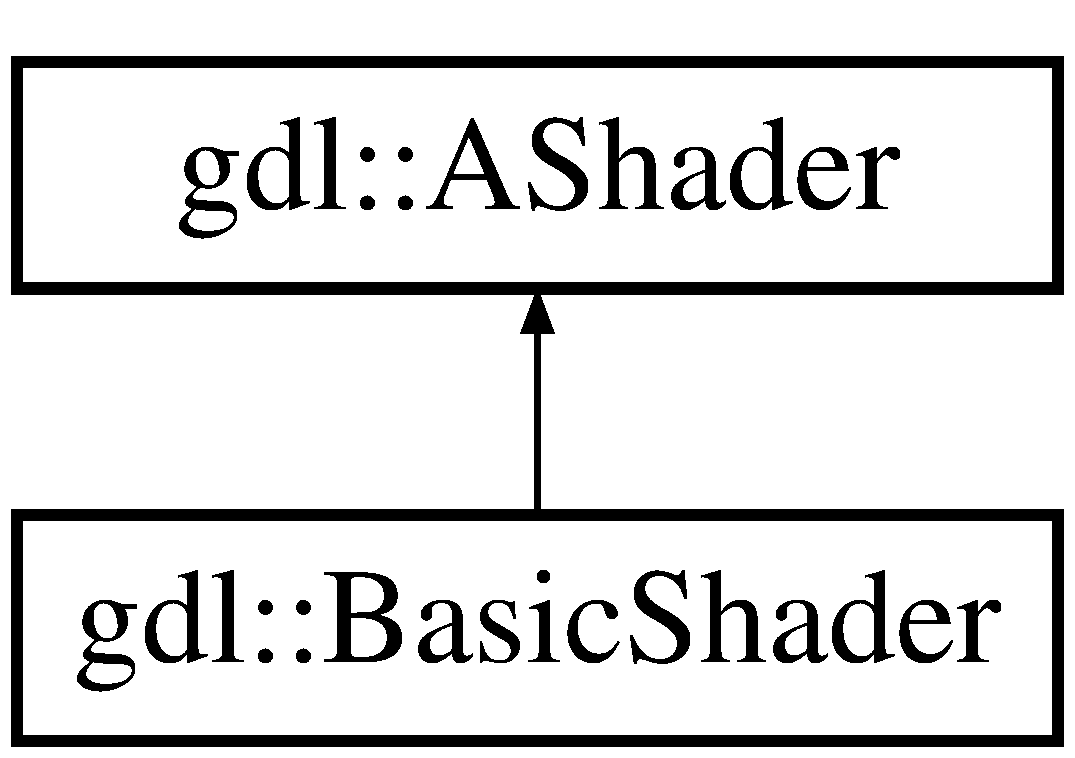
\includegraphics[height=2.000000cm]{classgdl_1_1_basic_shader}
\end{center}
\end{figure}
\subsection*{Public Member Functions}
\begin{DoxyCompactItemize}
\item 
virtual bool \hyperlink{classgdl_1_1_basic_shader_a2fbfee8bd2e95b001617bfe34c1e53e4}{build} ()
\begin{DoxyCompactList}\small\item\em Build and link the shader (using \-\_\-compile\-Shader and \-\_\-link) and bind the locations of the attributes and samplers. \end{DoxyCompactList}\end{DoxyCompactItemize}
\subsection*{Additional Inherited Members}


\subsection{Member Function Documentation}
\hypertarget{classgdl_1_1_basic_shader_a2fbfee8bd2e95b001617bfe34c1e53e4}{\index{gdl\-::\-Basic\-Shader@{gdl\-::\-Basic\-Shader}!build@{build}}
\index{build@{build}!gdl::BasicShader@{gdl\-::\-Basic\-Shader}}
\subsubsection[{build}]{\setlength{\rightskip}{0pt plus 5cm}bool gdl\-::\-Basic\-Shader\-::build (
\begin{DoxyParamCaption}
{}
\end{DoxyParamCaption}
)\hspace{0.3cm}{\ttfamily [virtual]}}}\label{classgdl_1_1_basic_shader_a2fbfee8bd2e95b001617bfe34c1e53e4}


Build and link the shader (using \-\_\-compile\-Shader and \-\_\-link) and bind the locations of the attributes and samplers. 

\begin{DoxyReturn}{Returns}
True if the build succeed, false otherwise. 
\end{DoxyReturn}


Implements \hyperlink{classgdl_1_1_a_shader_a0717c838d5a465332be5b91d12d2dbb5}{gdl\-::\-A\-Shader}.



The documentation for this class was generated from the following files\-:\begin{DoxyCompactItemize}
\item 
includes/Basic\-Shader.\-hh\item 
sources/Basic\-Shader.\-cpp\end{DoxyCompactItemize}

\hypertarget{classgdl_1_1_clock}{}\section{gdl\+:\+:Clock Class Reference}
\label{classgdl_1_1_clock}\index{gdl\+::\+Clock@{gdl\+::\+Clock}}
\subsection*{Public Member Functions}
\begin{DoxyCompactItemize}
\item 
\hypertarget{classgdl_1_1_clock_a1ec15565cb419cd67e6cdfedf6b112ca}{}\hyperlink{_s_d_l__audio_8h_a52835ae37c4bb905b903cbaf5d04b05f}{void} {\bfseries update} (unsigned \hyperlink{_s_d_l__thread_8h_a6a64f9be4433e4de6e2f2f548cf3c08e}{int} current\+Time)\label{classgdl_1_1_clock_a1ec15565cb419cd67e6cdfedf6b112ca}

\item 
\hypertarget{classgdl_1_1_clock_a8ea324bb269ca68e8f5a8c1cf071c3f7}{}double {\bfseries get\+Elapsed} () const \label{classgdl_1_1_clock_a8ea324bb269ca68e8f5a8c1cf071c3f7}

\end{DoxyCompactItemize}
\subsection*{Private Attributes}
\begin{DoxyCompactItemize}
\item 
\hypertarget{classgdl_1_1_clock_a4a8bc22ef6b697e47f7065db2bb6797f}{}unsigned \hyperlink{_s_d_l__thread_8h_a6a64f9be4433e4de6e2f2f548cf3c08e}{int} {\bfseries \+\_\+old\+Time}\label{classgdl_1_1_clock_a4a8bc22ef6b697e47f7065db2bb6797f}

\item 
\hypertarget{classgdl_1_1_clock_a6cca866f9dcfaabd8e0ac22660301398}{}unsigned \hyperlink{_s_d_l__thread_8h_a6a64f9be4433e4de6e2f2f548cf3c08e}{int} {\bfseries \+\_\+cur\+Time}\label{classgdl_1_1_clock_a6cca866f9dcfaabd8e0ac22660301398}

\end{DoxyCompactItemize}


The documentation for this class was generated from the following file\+:\begin{DoxyCompactItemize}
\item 
lib/gdl/includes/Clock.\+hh\end{DoxyCompactItemize}

\hypertarget{classgdl_1_1_game}{\section{gdl\-:\-:Game Class Reference}
\label{classgdl_1_1_game}\index{gdl\-::\-Game@{gdl\-::\-Game}}
}


It's your job to inherit from this and fill the abstract methods.  




{\ttfamily \#include $<$Game.\-hh$>$}

\subsection*{Public Member Functions}
\begin{DoxyCompactItemize}
\item 
\hypertarget{classgdl_1_1_game_aecd7b2ddca26bdea632cd2f7a0dc7b49}{virtual bool \hyperlink{classgdl_1_1_game_aecd7b2ddca26bdea632cd2f7a0dc7b49}{initialize} ()=0}\label{classgdl_1_1_game_aecd7b2ddca26bdea632cd2f7a0dc7b49}

\begin{DoxyCompactList}\small\item\em Pure virtual function used to initialize the game. \end{DoxyCompactList}\item 
\hypertarget{classgdl_1_1_game_a48f421b3d96140732cf028057feca989}{virtual bool \hyperlink{classgdl_1_1_game_a48f421b3d96140732cf028057feca989}{update} ()=0}\label{classgdl_1_1_game_a48f421b3d96140732cf028057feca989}

\begin{DoxyCompactList}\small\item\em Pure virtual function used to update the game logic. \end{DoxyCompactList}\item 
\hypertarget{classgdl_1_1_game_a3de59c743de1fc51cc464f0d47514ffa}{virtual void \hyperlink{classgdl_1_1_game_a3de59c743de1fc51cc464f0d47514ffa}{draw} ()=0}\label{classgdl_1_1_game_a3de59c743de1fc51cc464f0d47514ffa}

\begin{DoxyCompactList}\small\item\em Pure virtual function used to draw a frame. \end{DoxyCompactList}\end{DoxyCompactItemize}


\subsection{Detailed Description}
It's your job to inherit from this and fill the abstract methods. 

The documentation for this class was generated from the following files\-:\begin{DoxyCompactItemize}
\item 
includes/Game.\-hh\item 
sources/Game.\-cpp\end{DoxyCompactItemize}

\hypertarget{classgdl_1_1_geometry}{}\section{gdl\+:\+:Geometry Class Reference}
\label{classgdl_1_1_geometry}\index{gdl\+::\+Geometry@{gdl\+::\+Geometry}}
\subsection*{Public Member Functions}
\begin{DoxyCompactItemize}
\item 
\hypertarget{classgdl_1_1_geometry_a541c2b0d02cd3cbee44dbb312bd682f8}{}\hyperlink{classgdl_1_1_geometry}{Geometry} \& {\bfseries push\+Vertex} (const \hyperlink{group__core__types_gad45787527c6ff2bd6680867204eb0354}{glm\+::vec3} \&t)\label{classgdl_1_1_geometry_a541c2b0d02cd3cbee44dbb312bd682f8}

\item 
\hypertarget{classgdl_1_1_geometry_aa441f58a331324338c4001012d550690}{}\hyperlink{classgdl_1_1_geometry}{Geometry} \& {\bfseries push\+Uv} (const \hyperlink{group__core__types_ga66d091b759687504ab01365fbd33a1dd}{glm\+::vec2} \&t)\label{classgdl_1_1_geometry_aa441f58a331324338c4001012d550690}

\item 
\hypertarget{classgdl_1_1_geometry_aa727f26ba81f6fe814f9a47f8282ae33}{}\hyperlink{classgdl_1_1_geometry}{Geometry} \& {\bfseries push\+Normal} (const \hyperlink{group__core__types_gad45787527c6ff2bd6680867204eb0354}{glm\+::vec3} \&t)\label{classgdl_1_1_geometry_aa727f26ba81f6fe814f9a47f8282ae33}

\item 
\hypertarget{classgdl_1_1_geometry_a10c8f23c09c2c118038e5087ea767c07}{}\hyperlink{classgdl_1_1_geometry}{Geometry} \& {\bfseries set\+Color} (const \hyperlink{group__core__types_gae9c89157f980f7247cdee8bf55787035}{glm\+::vec4} \&t)\label{classgdl_1_1_geometry_a10c8f23c09c2c118038e5087ea767c07}

\item 
\hypertarget{classgdl_1_1_geometry_a6e8f3c283012d41ea72d4f091b82652d}{}bool {\bfseries build} ()\label{classgdl_1_1_geometry_a6e8f3c283012d41ea72d4f091b82652d}

\item 
\hypertarget{classgdl_1_1_geometry_a1345bc83eed3ae62fce3158e459e6973}{}\hyperlink{_s_d_l__audio_8h_a52835ae37c4bb905b903cbaf5d04b05f}{void} {\bfseries draw} (\hyperlink{classgdl_1_1_a_shader}{A\+Shader} \&shader, \hyperlink{group__core__types_ga7dcd2365c2e368e6af5b7adeb6a9c8df}{glm\+::mat4} const \&transform, G\+Lenum draw\+Mode)\label{classgdl_1_1_geometry_a1345bc83eed3ae62fce3158e459e6973}

\end{DoxyCompactItemize}
\subsection*{Private Attributes}
\begin{DoxyCompactItemize}
\item 
\hypertarget{classgdl_1_1_geometry_a701ce247c8e544e8016f8098acd1d1c1}{}Vertex\+Buffer $\ast$ {\bfseries \+\_\+buffer}\label{classgdl_1_1_geometry_a701ce247c8e544e8016f8098acd1d1c1}

\item 
\hypertarget{classgdl_1_1_geometry_ab4ed295013a720a3e871a4531c53245f}{}std\+::vector$<$ \hyperlink{group__core__types_gae9c89157f980f7247cdee8bf55787035}{glm\+::vec4} $>$ {\bfseries \+\_\+vertices}\label{classgdl_1_1_geometry_ab4ed295013a720a3e871a4531c53245f}

\item 
\hypertarget{classgdl_1_1_geometry_aa999936e3bc2bb7c7bc9e9314e2f2df8}{}std\+::vector$<$ \hyperlink{group__core__types_gae9c89157f980f7247cdee8bf55787035}{glm\+::vec4} $>$ {\bfseries \+\_\+colors}\label{classgdl_1_1_geometry_aa999936e3bc2bb7c7bc9e9314e2f2df8}

\item 
\hypertarget{classgdl_1_1_geometry_a41df7e65df7500fb1b83e09260b1c468}{}std\+::vector$<$ \hyperlink{group__core__types_gae9c89157f980f7247cdee8bf55787035}{glm\+::vec4} $>$ {\bfseries \+\_\+normals}\label{classgdl_1_1_geometry_a41df7e65df7500fb1b83e09260b1c468}

\item 
\hypertarget{classgdl_1_1_geometry_a0d0a522d32e09eada6d5803ec006ad61}{}std\+::vector$<$ \hyperlink{group__core__types_ga66d091b759687504ab01365fbd33a1dd}{glm\+::vec2} $>$ {\bfseries \+\_\+uvs}\label{classgdl_1_1_geometry_a0d0a522d32e09eada6d5803ec006ad61}

\item 
\hypertarget{classgdl_1_1_geometry_a2877b29791a47a9680c6d3a94eeeabd3}{}\hyperlink{group__core__types_gae9c89157f980f7247cdee8bf55787035}{glm\+::vec4} {\bfseries \+\_\+current\+Color}\label{classgdl_1_1_geometry_a2877b29791a47a9680c6d3a94eeeabd3}

\end{DoxyCompactItemize}


The documentation for this class was generated from the following file\+:\begin{DoxyCompactItemize}
\item 
lib/gdl/includes/Geometry.\+hh\end{DoxyCompactItemize}

\hypertarget{classgdl_1_1_input}{}\section{gdl\+:\+:Input Class Reference}
\label{classgdl_1_1_input}\index{gdl\+::\+Input@{gdl\+::\+Input}}
\subsection*{Public Member Functions}
\begin{DoxyCompactItemize}
\item 
\hypertarget{classgdl_1_1_input_a2cbd704d4c1069ac1fd7c4fb91d30b09}{}\hyperlink{_s_d_l__audio_8h_a52835ae37c4bb905b903cbaf5d04b05f}{void} {\bfseries clear\+Inputs} ()\label{classgdl_1_1_input_a2cbd704d4c1069ac1fd7c4fb91d30b09}

\item 
\hypertarget{classgdl_1_1_input_a7a175a63e780f1aa0fdebba68c0e8850}{}\hyperlink{_s_d_l__audio_8h_a52835ae37c4bb905b903cbaf5d04b05f}{void} {\bfseries add\+Input} (\hyperlink{_s_d_l__thread_8h_a6a64f9be4433e4de6e2f2f548cf3c08e}{int} input)\label{classgdl_1_1_input_a7a175a63e780f1aa0fdebba68c0e8850}

\item 
\hypertarget{classgdl_1_1_input_aa3380058a91f20b4889371ea07fd2bb4}{}\hyperlink{_s_d_l__audio_8h_a52835ae37c4bb905b903cbaf5d04b05f}{void} {\bfseries add\+Key\+Input} (\hyperlink{_s_d_l__thread_8h_a6a64f9be4433e4de6e2f2f548cf3c08e}{int} input)\label{classgdl_1_1_input_aa3380058a91f20b4889371ea07fd2bb4}

\item 
\hypertarget{classgdl_1_1_input_a531d2a805f5fdd33a0ce70ad74d0b3f8}{}\hyperlink{_s_d_l__audio_8h_a52835ae37c4bb905b903cbaf5d04b05f}{void} {\bfseries remove\+Key\+Input} (\hyperlink{_s_d_l__thread_8h_a6a64f9be4433e4de6e2f2f548cf3c08e}{int} input)\label{classgdl_1_1_input_a531d2a805f5fdd33a0ce70ad74d0b3f8}

\item 
\hypertarget{classgdl_1_1_input_aa6be10489840280271415ec1311ce5af}{}\hyperlink{_s_d_l__audio_8h_a52835ae37c4bb905b903cbaf5d04b05f}{void} {\bfseries set\+Mouse\+Position} (\hyperlink{group__core__types_ga606b9d298d8aaa55c449182c340b4622}{glm\+::ivec2} const \&pos, \hyperlink{group__core__types_ga606b9d298d8aaa55c449182c340b4622}{glm\+::ivec2} const \&rel)\label{classgdl_1_1_input_aa6be10489840280271415ec1311ce5af}

\item 
\hypertarget{classgdl_1_1_input_a4864b681a18a087443024160861587fb}{}\hyperlink{_s_d_l__audio_8h_a52835ae37c4bb905b903cbaf5d04b05f}{void} {\bfseries set\+Mouse\+Wheel} (\hyperlink{group__core__types_ga606b9d298d8aaa55c449182c340b4622}{glm\+::ivec2} const \&delta)\label{classgdl_1_1_input_a4864b681a18a087443024160861587fb}

\item 
\hypertarget{classgdl_1_1_input_a7106c72dc65072969c2cfd7225b63e72}{}\hyperlink{group__core__types_ga606b9d298d8aaa55c449182c340b4622}{glm\+::ivec2} const \& {\bfseries get\+Mouse\+Position} ()\label{classgdl_1_1_input_a7106c72dc65072969c2cfd7225b63e72}

\item 
\hypertarget{classgdl_1_1_input_a7a140bee02c1d841f1d31fc088da09a9}{}\hyperlink{group__core__types_ga606b9d298d8aaa55c449182c340b4622}{glm\+::ivec2} const \& {\bfseries get\+Mouse\+Delta} ()\label{classgdl_1_1_input_a7a140bee02c1d841f1d31fc088da09a9}

\item 
\hypertarget{classgdl_1_1_input_a5abcc6f6e15e0567e6edc245b379a3ad}{}\hyperlink{group__core__types_ga606b9d298d8aaa55c449182c340b4622}{glm\+::ivec2} const \& {\bfseries get\+Mouse\+Wheel} ()\label{classgdl_1_1_input_a5abcc6f6e15e0567e6edc245b379a3ad}

\item 
\hypertarget{classgdl_1_1_input_a7d26a492aaf056166fe64ec00a927b7a}{}bool {\bfseries get\+Input} (\hyperlink{_s_d_l__thread_8h_a6a64f9be4433e4de6e2f2f548cf3c08e}{int} input, bool handled=false)\label{classgdl_1_1_input_a7d26a492aaf056166fe64ec00a927b7a}

\item 
\hypertarget{classgdl_1_1_input_a8edd2ea49ebf6c8a833a65cf80133c4c}{}bool {\bfseries get\+Key} (\hyperlink{_s_d_l__thread_8h_a6a64f9be4433e4de6e2f2f548cf3c08e}{int} input, bool handled=false)\label{classgdl_1_1_input_a8edd2ea49ebf6c8a833a65cf80133c4c}

\item 
\hypertarget{classgdl_1_1_input_ae91c9e623df178477454a6e8a543a821}{}bool {\bfseries get\+Key\+Down} (\hyperlink{_s_d_l__thread_8h_a6a64f9be4433e4de6e2f2f548cf3c08e}{int} input, bool handled=false)\label{classgdl_1_1_input_ae91c9e623df178477454a6e8a543a821}

\item 
\hypertarget{classgdl_1_1_input_a51be7c3b3d47acc49745813cce736a78}{}bool {\bfseries get\+Key\+Up} (\hyperlink{_s_d_l__thread_8h_a6a64f9be4433e4de6e2f2f548cf3c08e}{int} input, bool handled=false)\label{classgdl_1_1_input_a51be7c3b3d47acc49745813cce736a78}

\end{DoxyCompactItemize}
\subsection*{Private Attributes}
\begin{DoxyCompactItemize}
\item 
\hypertarget{classgdl_1_1_input_a5ea5785adf82a05ba063db0eabdbbdec}{}std\+::list$<$ \hyperlink{_s_d_l__thread_8h_a6a64f9be4433e4de6e2f2f548cf3c08e}{int} $>$ {\bfseries \+\_\+inputs}\label{classgdl_1_1_input_a5ea5785adf82a05ba063db0eabdbbdec}

\item 
\hypertarget{classgdl_1_1_input_adeee18a4c305853daac3b43e6318f244}{}std\+::list$<$ \hyperlink{_s_d_l__thread_8h_a6a64f9be4433e4de6e2f2f548cf3c08e}{int} $>$ {\bfseries \+\_\+key\+Inputs}\label{classgdl_1_1_input_adeee18a4c305853daac3b43e6318f244}

\item 
\hypertarget{classgdl_1_1_input_a3e88cc5cafd06d625b4e553f96b500eb}{}\hyperlink{group__core__types_ga606b9d298d8aaa55c449182c340b4622}{glm\+::ivec2} {\bfseries \+\_\+mouse\+Position}\label{classgdl_1_1_input_a3e88cc5cafd06d625b4e553f96b500eb}

\item 
\hypertarget{classgdl_1_1_input_a11cc55c61d6a00d9b83632aeeeeed594}{}\hyperlink{group__core__types_ga606b9d298d8aaa55c449182c340b4622}{glm\+::ivec2} {\bfseries \+\_\+mouse\+Delta}\label{classgdl_1_1_input_a11cc55c61d6a00d9b83632aeeeeed594}

\item 
\hypertarget{classgdl_1_1_input_a20209fae01946c5ff185d67b8c9d4b39}{}\hyperlink{group__core__types_ga606b9d298d8aaa55c449182c340b4622}{glm\+::ivec2} {\bfseries \+\_\+mouse\+Wheel\+Delta}\label{classgdl_1_1_input_a20209fae01946c5ff185d67b8c9d4b39}

\end{DoxyCompactItemize}


The documentation for this class was generated from the following file\+:\begin{DoxyCompactItemize}
\item 
lib/gdl/includes/Input.\+hh\end{DoxyCompactItemize}

\hypertarget{classgdl_1_1_i_render_context}{}\section{gdl\+:\+:I\+Render\+Context Class Reference}
\label{classgdl_1_1_i_render_context}\index{gdl\+::\+I\+Render\+Context@{gdl\+::\+I\+Render\+Context}}


Inheritance diagram for gdl\+:\+:I\+Render\+Context\+:
% FIG 0
\subsection*{Public Member Functions}
\begin{DoxyCompactItemize}
\item 
\hypertarget{classgdl_1_1_i_render_context_a962fd24dc84758aaa7c7d28330c3e37e}{}virtual bool {\bfseries start} (unsigned \hyperlink{_s_d_l__thread_8h_a6a64f9be4433e4de6e2f2f548cf3c08e}{int} swidth, unsigned \hyperlink{_s_d_l__thread_8h_a6a64f9be4433e4de6e2f2f548cf3c08e}{int} sheight, const std\+::string \&name, \hyperlink{_s_d_l__thread_8h_a6a64f9be4433e4de6e2f2f548cf3c08e}{int} init\+Flags, \hyperlink{_s_d_l__thread_8h_a6a64f9be4433e4de6e2f2f548cf3c08e}{int} windows\+Flags)=0\label{classgdl_1_1_i_render_context_a962fd24dc84758aaa7c7d28330c3e37e}

\item 
\hypertarget{classgdl_1_1_i_render_context_a19ffcdcc82d88098693a08f66beab770}{}virtual \hyperlink{_s_d_l__audio_8h_a52835ae37c4bb905b903cbaf5d04b05f}{void} {\bfseries update\+Inputs} (\hyperlink{classgdl_1_1_input}{Input} \&input) const =0\label{classgdl_1_1_i_render_context_a19ffcdcc82d88098693a08f66beab770}

\item 
\hypertarget{classgdl_1_1_i_render_context_af2134a929634632ccf13e779f489cdc2}{}virtual \hyperlink{_s_d_l__audio_8h_a52835ae37c4bb905b903cbaf5d04b05f}{void} {\bfseries update\+Clock} (\hyperlink{classgdl_1_1_clock}{Clock} \&clock) const =0\label{classgdl_1_1_i_render_context_af2134a929634632ccf13e779f489cdc2}

\item 
\hypertarget{classgdl_1_1_i_render_context_aa7ad85ff39d1e82f25162b71284b3659}{}virtual \hyperlink{_s_d_l__audio_8h_a52835ae37c4bb905b903cbaf5d04b05f}{void} {\bfseries flush} () const =0\label{classgdl_1_1_i_render_context_aa7ad85ff39d1e82f25162b71284b3659}

\item 
\hypertarget{classgdl_1_1_i_render_context_af1f487e928504f86f878f904fb4075cf}{}virtual \hyperlink{_s_d_l__audio_8h_a52835ae37c4bb905b903cbaf5d04b05f}{void} {\bfseries stop} () const =0\label{classgdl_1_1_i_render_context_af1f487e928504f86f878f904fb4075cf}

\end{DoxyCompactItemize}


The documentation for this class was generated from the following file\+:\begin{DoxyCompactItemize}
\item 
lib/gdl/includes/I\+Render\+Context.\+hh\end{DoxyCompactItemize}

\hypertarget{classgdl_1_1_model}{}\section{gdl\+:\+:Model Class Reference}
\label{classgdl_1_1_model}\index{gdl\+::\+Model@{gdl\+::\+Model}}
\subsection*{Public Member Functions}
\begin{DoxyCompactItemize}
\item 
\hypertarget{classgdl_1_1_model_a2880a8151a0a076dccc17c8a12530dcc}{}\hyperlink{_s_d_l__audio_8h_a52835ae37c4bb905b903cbaf5d04b05f}{void} {\bfseries pause} (bool pause\+Anim)\label{classgdl_1_1_model_a2880a8151a0a076dccc17c8a12530dcc}

\item 
\hypertarget{classgdl_1_1_model_a223b04dc9a2007ac22cc71d019af5749}{}bool {\bfseries set\+Current\+Anim} (\hyperlink{_s_d_l__thread_8h_a6a64f9be4433e4de6e2f2f548cf3c08e}{int} stack, bool loop=true)\label{classgdl_1_1_model_a223b04dc9a2007ac22cc71d019af5749}

\item 
\hypertarget{classgdl_1_1_model_ac4210edf1cfc619f8948e83820b41ca9}{}bool {\bfseries set\+Current\+Anim} (std\+::string const \&name, bool loop=true)\label{classgdl_1_1_model_ac4210edf1cfc619f8948e83820b41ca9}

\item 
\hypertarget{classgdl_1_1_model_a6c07ff9af9e5f21976f74c76969c5209}{}\hyperlink{_s_d_l__thread_8h_a6a64f9be4433e4de6e2f2f548cf3c08e}{int} {\bfseries get\+Animation\+Frame\+Number} (\hyperlink{_s_d_l__thread_8h_a6a64f9be4433e4de6e2f2f548cf3c08e}{int} stack)\label{classgdl_1_1_model_a6c07ff9af9e5f21976f74c76969c5209}

\item 
\hypertarget{classgdl_1_1_model_a2f46e23c1f5bbf46724ab88d4e09edeb}{}\hyperlink{_s_d_l__thread_8h_a6a64f9be4433e4de6e2f2f548cf3c08e}{int} {\bfseries get\+Animation\+Frame\+Number} (std\+::string const \&name)\label{classgdl_1_1_model_a2f46e23c1f5bbf46724ab88d4e09edeb}

\item 
\hypertarget{classgdl_1_1_model_a145f9bb956d043c28f23d8714e72447c}{}float {\bfseries get\+Frame\+Duration} ()\label{classgdl_1_1_model_a145f9bb956d043c28f23d8714e72447c}

\item 
\hypertarget{classgdl_1_1_model_ac903e3a9a4da067bf245a26e4bb02fd0}{}bool {\bfseries create\+Sub\+Anim} (\hyperlink{_s_d_l__thread_8h_a6a64f9be4433e4de6e2f2f548cf3c08e}{int} stack, std\+::string const \&sub\+Anim\+Name, \hyperlink{_s_d_l__thread_8h_a6a64f9be4433e4de6e2f2f548cf3c08e}{int} frame\+Start, \hyperlink{_s_d_l__thread_8h_a6a64f9be4433e4de6e2f2f548cf3c08e}{int} frame\+End)\label{classgdl_1_1_model_ac903e3a9a4da067bf245a26e4bb02fd0}

\item 
\hypertarget{classgdl_1_1_model_aa712f9125986a0d0ee9520e73a2a0f66}{}bool {\bfseries create\+Sub\+Anim} (std\+::string const \&name, std\+::string const \&sub\+Anim\+Name, \hyperlink{_s_d_l__thread_8h_a6a64f9be4433e4de6e2f2f548cf3c08e}{int} frame\+Start, \hyperlink{_s_d_l__thread_8h_a6a64f9be4433e4de6e2f2f548cf3c08e}{int} frame\+End)\label{classgdl_1_1_model_aa712f9125986a0d0ee9520e73a2a0f66}

\item 
\hypertarget{classgdl_1_1_model_a7167ca64cd426f7bd46756ed33bad12f}{}bool {\bfseries set\+Current\+Sub\+Anim} (std\+::string const \&name, bool loop=true)\label{classgdl_1_1_model_a7167ca64cd426f7bd46756ed33bad12f}

\item 
\hypertarget{classgdl_1_1_model_a73175b246228b1a275a4cf2b59c8d5cd}{}bool {\bfseries load} (std\+::string const \&path)\label{classgdl_1_1_model_a73175b246228b1a275a4cf2b59c8d5cd}

\item 
\hypertarget{classgdl_1_1_model_a57be549452c2bef282709fe02b0072a3}{}\hyperlink{_s_d_l__audio_8h_a52835ae37c4bb905b903cbaf5d04b05f}{void} {\bfseries draw} (\hyperlink{classgdl_1_1_a_shader}{A\+Shader} \&shader, \hyperlink{group__core__types_ga7dcd2365c2e368e6af5b7adeb6a9c8df}{glm\+::mat4} const \&transform, double delta\+Time)\label{classgdl_1_1_model_a57be549452c2bef282709fe02b0072a3}

\end{DoxyCompactItemize}
\subsection*{Private Member Functions}
\begin{DoxyCompactItemize}
\item 
\hypertarget{classgdl_1_1_model_a27dfe1058071caf1285b305ae6c9f5ff}{}\hyperlink{_s_d_l__audio_8h_a52835ae37c4bb905b903cbaf5d04b05f}{void} {\bfseries remove\+From\+Manager} ()\label{classgdl_1_1_model_a27dfe1058071caf1285b305ae6c9f5ff}

\end{DoxyCompactItemize}
\subsection*{Private Attributes}
\begin{DoxyCompactItemize}
\item 
\hypertarget{classgdl_1_1_model_a77abc5e28c6bb239efe898c63312fa2f}{}Fbx\+Model $\ast$ {\bfseries \+\_\+model}\label{classgdl_1_1_model_a77abc5e28c6bb239efe898c63312fa2f}

\item 
\hypertarget{classgdl_1_1_model_a93a620a2af97597fb545f86dd236063a}{}S\+Fbx\+Model\+Handler $\ast$ {\bfseries \+\_\+model\+Handler}\label{classgdl_1_1_model_a93a620a2af97597fb545f86dd236063a}

\item 
\hypertarget{classgdl_1_1_model_a5c801dcd2b17b692c9762f5a76a53e65}{}bool {\bfseries \+\_\+loop}\label{classgdl_1_1_model_a5c801dcd2b17b692c9762f5a76a53e65}

\item 
\hypertarget{classgdl_1_1_model_a6513f5a017d5a0a542372522b2f1781b}{}double {\bfseries \+\_\+time\+Since\+Last\+Frame}\label{classgdl_1_1_model_a6513f5a017d5a0a542372522b2f1781b}

\item 
\hypertarget{classgdl_1_1_model_aa97070e9962ec6b5f86d55ab642b7025}{}std\+::map$<$ std\+::string, S\+Sub\+Animation\+Datas $>$ {\bfseries \+\_\+sub\+Anims}\label{classgdl_1_1_model_aa97070e9962ec6b5f86d55ab642b7025}

\end{DoxyCompactItemize}
\subsection*{Static Private Attributes}
\begin{DoxyCompactItemize}
\item 
\hypertarget{classgdl_1_1_model_adbb05700333f09f60d288734fe9a6eaa}{}static std\+::map$<$ std\+::string, S\+Fbx\+Model\+Handler $\ast$ $>$ {\bfseries \+\_\+mesh\+Manager}\label{classgdl_1_1_model_adbb05700333f09f60d288734fe9a6eaa}

\end{DoxyCompactItemize}


The documentation for this class was generated from the following file\+:\begin{DoxyCompactItemize}
\item 
lib/gdl/includes/Model.\+hh\end{DoxyCompactItemize}

\hypertarget{classgdl_1_1_sdl_context}{\section{gdl\-:\-:Sdl\-Context Class Reference}
\label{classgdl_1_1_sdl_context}\index{gdl\-::\-Sdl\-Context@{gdl\-::\-Sdl\-Context}}
}


Class for an Sdl Context.  




{\ttfamily \#include $<$Sdl\-Context.\-hh$>$}

Inheritance diagram for gdl\-:\-:Sdl\-Context\-:\begin{figure}[H]
\begin{center}
\leavevmode
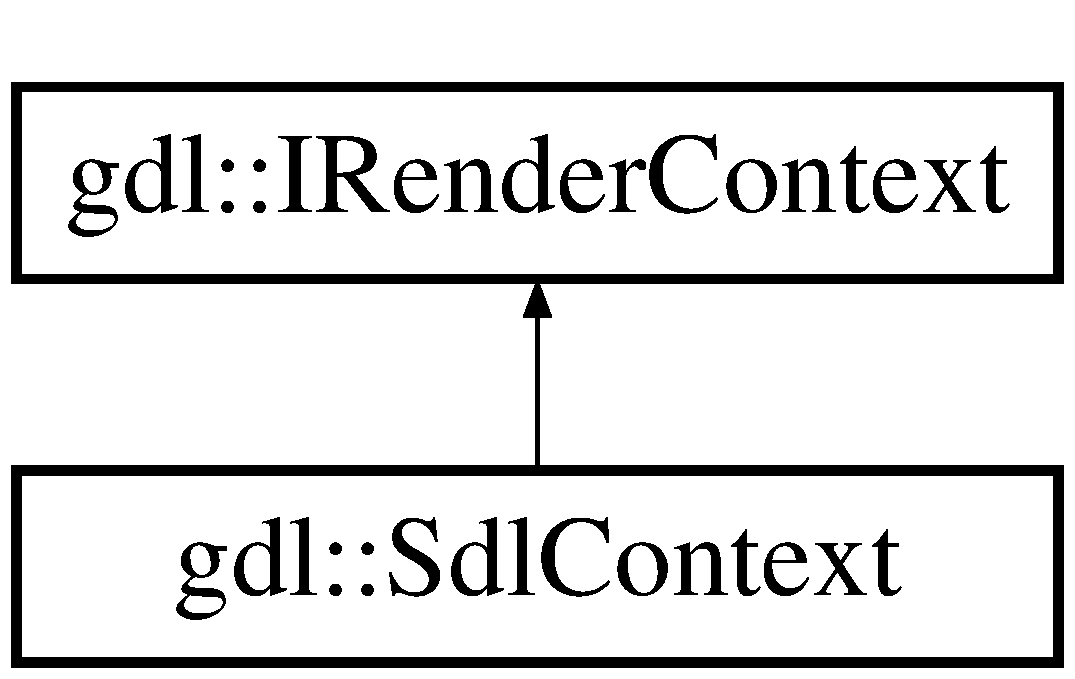
\includegraphics[height=2.000000cm]{classgdl_1_1_sdl_context}
\end{center}
\end{figure}
\subsection*{Public Member Functions}
\begin{DoxyCompactItemize}
\item 
virtual bool \hyperlink{classgdl_1_1_sdl_context_a317e2f02518809a4ff1d4ec381cf29a2}{start} (unsigned int swidth, unsigned int sheight, const std\-::string \&name, int init\-Flags=S\-D\-L\-\_\-\-I\-N\-I\-T\-\_\-\-V\-I\-D\-E\-O, int windows\-Flags=S\-D\-L\-\_\-\-W\-I\-N\-D\-O\-W\-\_\-\-O\-P\-E\-N\-G\-L)
\begin{DoxyCompactList}\small\item\em Start the context, create a window. \end{DoxyCompactList}\item 
virtual void \hyperlink{classgdl_1_1_sdl_context_a899be84a90438d59547155e4aecc2c87}{update\-Inputs} (\hyperlink{classgdl_1_1_input}{Input} \&input) const 
\begin{DoxyCompactList}\small\item\em Update the inputs. \end{DoxyCompactList}\item 
virtual void \hyperlink{classgdl_1_1_sdl_context_aec8807a2f1b9ca64c880286f1046ad2a}{update\-Clock} (\hyperlink{classgdl_1_1_clock}{Clock} \&clock) const 
\begin{DoxyCompactList}\small\item\em Update the game clock. \end{DoxyCompactList}\item 
\hypertarget{classgdl_1_1_sdl_context_a107b456e3df4727c6c32fff36f45faa7}{virtual void \hyperlink{classgdl_1_1_sdl_context_a107b456e3df4727c6c32fff36f45faa7}{flush} () const }\label{classgdl_1_1_sdl_context_a107b456e3df4727c6c32fff36f45faa7}

\begin{DoxyCompactList}\small\item\em Flush the screen to show what has been drawn. (Just call S\-D\-L\-\_\-\-G\-L\-\_\-\-Swap\-Window). \end{DoxyCompactList}\item 
\hypertarget{classgdl_1_1_sdl_context_a02007ea70c7e5a60048c1bb5812b48b6}{virtual void \hyperlink{classgdl_1_1_sdl_context_a02007ea70c7e5a60048c1bb5812b48b6}{stop} () const }\label{classgdl_1_1_sdl_context_a02007ea70c7e5a60048c1bb5812b48b6}

\begin{DoxyCompactList}\small\item\em Close the context and the window. \end{DoxyCompactList}\end{DoxyCompactItemize}
\subsection*{Protected Attributes}
\begin{DoxyCompactItemize}
\item 
\hypertarget{classgdl_1_1_sdl_context_a3c298835a8a3e236d389efeb6c1d3303}{S\-D\-L\-\_\-\-Window $\ast$ \hyperlink{classgdl_1_1_sdl_context_a3c298835a8a3e236d389efeb6c1d3303}{\-\_\-window}}\label{classgdl_1_1_sdl_context_a3c298835a8a3e236d389efeb6c1d3303}

\begin{DoxyCompactList}\small\item\em The S\-D\-L window object. \end{DoxyCompactList}\item 
\hypertarget{classgdl_1_1_sdl_context_a8a997eff1d38bc784ee95ce76db93359}{S\-D\-L\-\_\-\-G\-L\-Context \hyperlink{classgdl_1_1_sdl_context_a8a997eff1d38bc784ee95ce76db93359}{\-\_\-gl\-Context}}\label{classgdl_1_1_sdl_context_a8a997eff1d38bc784ee95ce76db93359}

\begin{DoxyCompactList}\small\item\em The S\-D\-L Open\-G\-L context object. \end{DoxyCompactList}\end{DoxyCompactItemize}


\subsection{Detailed Description}
Class for an Sdl Context. 

\subsection{Member Function Documentation}
\hypertarget{classgdl_1_1_sdl_context_a317e2f02518809a4ff1d4ec381cf29a2}{\index{gdl\-::\-Sdl\-Context@{gdl\-::\-Sdl\-Context}!start@{start}}
\index{start@{start}!gdl::SdlContext@{gdl\-::\-Sdl\-Context}}
\subsubsection[{start}]{\setlength{\rightskip}{0pt plus 5cm}bool gdl\-::\-Sdl\-Context\-::start (
\begin{DoxyParamCaption}
\item[{unsigned int}]{swidth, }
\item[{unsigned int}]{sheight, }
\item[{const std\-::string \&}]{name, }
\item[{int}]{init\-Flags = {\ttfamily SDL\-\_\-INIT\-\_\-VIDEO}, }
\item[{int}]{windows\-Flags = {\ttfamily SDL\-\_\-WINDOW\-\_\-OPENGL}}
\end{DoxyParamCaption}
)\hspace{0.3cm}{\ttfamily [virtual]}}}\label{classgdl_1_1_sdl_context_a317e2f02518809a4ff1d4ec381cf29a2}


Start the context, create a window. 


\begin{DoxyParams}{Parameters}
{\em swidth} & The width of the window to create. \\
\hline
{\em sheight} & The height of the window to create. \\
\hline
{\em name} & The name of the window. \\
\hline
{\em init\-Flags} & Flags passed to S\-D\-L\-\_\-\-Init. \\
\hline
{\em windows\-Flags} & Flags passed to S\-D\-L\-\_\-\-Create\-Window. \\
\hline
\end{DoxyParams}
\begin{DoxyReturn}{Returns}
False if the context creation has failed. 
\end{DoxyReturn}


Implements \hyperlink{classgdl_1_1_i_render_context}{gdl\-::\-I\-Render\-Context}.

\hypertarget{classgdl_1_1_sdl_context_aec8807a2f1b9ca64c880286f1046ad2a}{\index{gdl\-::\-Sdl\-Context@{gdl\-::\-Sdl\-Context}!update\-Clock@{update\-Clock}}
\index{update\-Clock@{update\-Clock}!gdl::SdlContext@{gdl\-::\-Sdl\-Context}}
\subsubsection[{update\-Clock}]{\setlength{\rightskip}{0pt plus 5cm}void gdl\-::\-Sdl\-Context\-::update\-Clock (
\begin{DoxyParamCaption}
\item[{{\bf Clock} \&}]{clock}
\end{DoxyParamCaption}
) const\hspace{0.3cm}{\ttfamily [virtual]}}}\label{classgdl_1_1_sdl_context_aec8807a2f1b9ca64c880286f1046ad2a}


Update the game clock. 


\begin{DoxyParams}{Parameters}
{\em input} & The clock object to update. \\
\hline
\end{DoxyParams}


Implements \hyperlink{classgdl_1_1_i_render_context}{gdl\-::\-I\-Render\-Context}.

\hypertarget{classgdl_1_1_sdl_context_a899be84a90438d59547155e4aecc2c87}{\index{gdl\-::\-Sdl\-Context@{gdl\-::\-Sdl\-Context}!update\-Inputs@{update\-Inputs}}
\index{update\-Inputs@{update\-Inputs}!gdl::SdlContext@{gdl\-::\-Sdl\-Context}}
\subsubsection[{update\-Inputs}]{\setlength{\rightskip}{0pt plus 5cm}void gdl\-::\-Sdl\-Context\-::update\-Inputs (
\begin{DoxyParamCaption}
\item[{{\bf Input} \&}]{input}
\end{DoxyParamCaption}
) const\hspace{0.3cm}{\ttfamily [virtual]}}}\label{classgdl_1_1_sdl_context_a899be84a90438d59547155e4aecc2c87}


Update the inputs. 


\begin{DoxyParams}{Parameters}
{\em input} & The input object to fill. \\
\hline
\end{DoxyParams}


Implements \hyperlink{classgdl_1_1_i_render_context}{gdl\-::\-I\-Render\-Context}.



The documentation for this class was generated from the following files\-:\begin{DoxyCompactItemize}
\item 
includes/Sdl\-Context.\-hh\item 
sources/Sdl\-Context.\-cpp\end{DoxyCompactItemize}

\hypertarget{classgdl_1_1_texture}{}\section{gdl\+:\+:Texture Class Reference}
\label{classgdl_1_1_texture}\index{gdl\+::\+Texture@{gdl\+::\+Texture}}
\subsection*{Public Member Functions}
\begin{DoxyCompactItemize}
\item 
\hypertarget{classgdl_1_1_texture_a2d010f85c81be8c5b19cf7b4f0ae1af0}{}{\bfseries Texture} (\hyperlink{classgdl_1_1_texture}{Texture} const \&o)\label{classgdl_1_1_texture_a2d010f85c81be8c5b19cf7b4f0ae1af0}

\item 
\hypertarget{classgdl_1_1_texture_ada7dffc24ec794f7cc5a5a26dc0261fc}{}bool {\bfseries load} (const std\+::string \&path, bool gen\+Mimaps=false)\label{classgdl_1_1_texture_ada7dffc24ec794f7cc5a5a26dc0261fc}

\item 
\hypertarget{classgdl_1_1_texture_a1954740f65f3e9265d6f4506ec75f4c2}{}G\+Luint {\bfseries get\+Id} () const \label{classgdl_1_1_texture_a1954740f65f3e9265d6f4506ec75f4c2}

\item 
\hypertarget{classgdl_1_1_texture_a5b628612f89e1fc67a28085158236d9c}{}\hyperlink{_s_d_l__audio_8h_a52835ae37c4bb905b903cbaf5d04b05f}{void} {\bfseries bind} () const \label{classgdl_1_1_texture_a5b628612f89e1fc67a28085158236d9c}

\item 
\hypertarget{classgdl_1_1_texture_a932fca1cf9da4570df0591ae2272f545}{}G\+Luint {\bfseries get\+Width} () const \label{classgdl_1_1_texture_a932fca1cf9da4570df0591ae2272f545}

\item 
\hypertarget{classgdl_1_1_texture_a7ffaf22e021293cab2a856c2ec795dca}{}G\+Luint {\bfseries get\+Height} () const \label{classgdl_1_1_texture_a7ffaf22e021293cab2a856c2ec795dca}

\item 
\hypertarget{classgdl_1_1_texture_a54bb80c56d1969ed6deb69810a82a6ca}{}\hyperlink{classgdl_1_1_texture}{Texture} \& {\bfseries operator=} (\hyperlink{classgdl_1_1_texture}{Texture} const \&o)\label{classgdl_1_1_texture_a54bb80c56d1969ed6deb69810a82a6ca}

\end{DoxyCompactItemize}
\subsection*{Protected Attributes}
\begin{DoxyCompactItemize}
\item 
\hypertarget{classgdl_1_1_texture_a649311ec115dcd70df025714d52f887e}{}G\+Luint {\bfseries \+\_\+width}\label{classgdl_1_1_texture_a649311ec115dcd70df025714d52f887e}

\item 
\hypertarget{classgdl_1_1_texture_ad016a8f5410560f0ac2498eb75ba7570}{}G\+Luint {\bfseries \+\_\+height}\label{classgdl_1_1_texture_ad016a8f5410560f0ac2498eb75ba7570}

\item 
\hypertarget{classgdl_1_1_texture_ad583257567501c6c9f58b943c03cde68}{}G\+Luint {\bfseries \+\_\+id}\label{classgdl_1_1_texture_ad583257567501c6c9f58b943c03cde68}

\end{DoxyCompactItemize}


The documentation for this class was generated from the following file\+:\begin{DoxyCompactItemize}
\item 
lib/gdl/includes/Texture.\+hh\end{DoxyCompactItemize}

%--- End generated contents ---

% Index
\newpage
\phantomsection
\addcontentsline{toc}{chapter}{Index}
\printindex

\end{document}
